\documentclass[11pt]{article}
\title{Assignment 6: Latex G5}
\author{Group 5: Alexandros Tsiridis, Stamatis Maritsas, Andray Afanasyev}
\date{}
\usepackage{url}
\usepackage{graphicx} 
\usepackage{placeins}
\addtolength{\oddsidemargin}{-.875in}
\addtolength{\evensidemargin}{-.875in}
\addtolength{\textwidth}{1.75in}
\addtolength{\topmargin}{-.875in}
\addtolength{\textheight}{1.75in}
\begin{document}
\maketitle

\nocite{*}
\section{Overhauling Amd for the ’00s: A Case Study of GNU Autotools}
\subsection{Introduction}
As group 5 we were assigned to look at the above article and discuss it during the lecture. In the following section, I am going to discuss about the article and what information I believe is useful to grasp from the paper, and what I learned from it. First of all, I will break up the article in three parts:
\begin{enumerate}
\item How the build was done before the autotools and what autotools have to offer.
\item Measuring complexity.
\item What you can gain by the use of autotools.
\end{enumerate}
\subsection{How the build was done before the autotools and what autotools have to offer}
Without the use of autotools, the building and configuration of the package is being done manually by the user and the programmer of it. At the first step, users have to manually configure a package before the compilation by changing the header file. In order to achieve this goal, the user need to have intimate knowledge of the system that he was trying to install the package on.

Moreover, in order for the programmers to achieve desired compatibility for the packages they are making use of extended CPP macros. These macros are being used to recognize features that the operating system need to have due to them being dependencies of the package. Such macros are complicated to write and usually end up in an extended nested form. Due to the complexity of the macros and their nested forms, maintenance of the package by the programmers becomes a nightmare.

Another way that is being used is the Imake utility which is designed specifically for building X11 applications. This tool defines static configurations for various systems, which cannot be account for local changes made by the user. One more utility which is being used is Metaconfig. This utility executes simple tests to find out the features of the system, but needs a lot of interaction with the user to confirm that the detection is correct.

GNU autotools were created in order to address the problems that were mentioned above. This is achieved by providing in build tests to dynamically detect various features of the system that are needed for the package. It is a suite of three tools namely Autoconf, Automake and Libtool.

\subsection{Measuring complexity}
In this subsection I am going to talk about three ways of measuring complexity that were mentioned in the article. I find these information quite useful even if someone is not interested in autotools or how to build a package without the use of them. In the paper, the three ways of measurement are:
\begin{itemize}
\item Measuring complexity according to the amount of the code lines inside the package.
\item Measuring complexity according to the amount of total CPP macros across the whole package.
\item Measuring complexity according to the average of total CPP macros per 1000 lines of code.
\end{itemize}

The first measurement will obviously make the biggest package the most complex. In my opinion, this is not an accurate way of measuring complexity as a bigger package might actually be less complex than a smaller one.

\begin{figure}[!htb]
\centering
  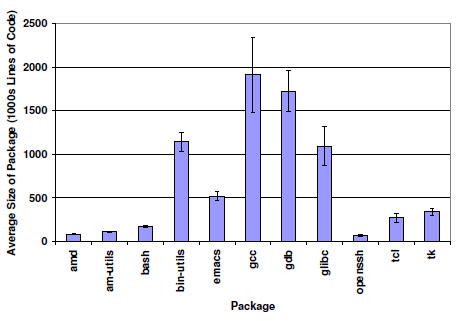
\includegraphics[width=.7\linewidth]{images/measure1}
  \caption{Average size of packages in thousands of lines of
code \cite{zadok2002}}
  \label{fig:measure1}
\end{figure}
\FloatBarrier
The second measurement its a bit more accurate than the way discussed above. It also has a fault as bigger packages usually tend to have more CPP conditionals than the smaller ones making them candidates for being the most complex ones in this measurement.

\begin{figure}[!htb]
\centering
  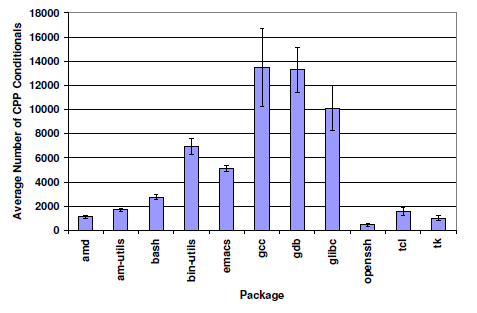
\includegraphics[width=.7\linewidth]{images/measure2}
  \caption{Average number of CPP conditionals per package \cite{zadok2002}}
  \label{fig:measure2}
\end{figure}
\FloatBarrier

The third measurement in my opinion, is better than the above two as it actually counts how often CPP commands are introduced inside the code.

\begin{figure}[!htb]
\centering
  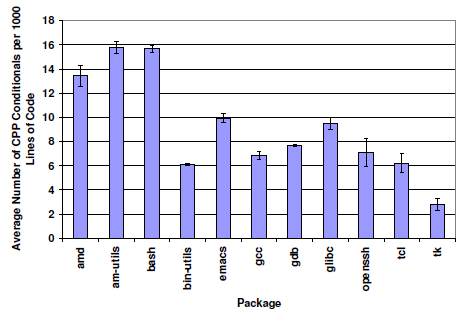
\includegraphics[width=.7\linewidth]{images/measure3}
  \caption{Average number of CPP conditionals per 1000 lines
of code \cite{zadok2002}}
  \label{fig:measure3}
\end{figure}
\FloatBarrier
To sum up, let's take the packages example seeing in the figures of gcc and amd. In the first figure, gcc climbs to the top of the complexity scale as the biggest package and amd is second from last due to its small size. In the second measurement, gcc is also the most complex one by a small difference from gdb and amd is third from last. And at the last measurement, where the size of the package does not actually matter, gcc is fourth in complexity from last and amd climbs to the third most complex package.

\subsection{What you can gain by the use of autotools}
By the use of autotools there are various benefits as well as a few disadvantages that are introduced. First of all, they reduce the complexity of code by automating the feature discovery procedure. They minimize the use of CPP conditionals by providing those in build tests. On the other hand, they do not reduce to zero the usage of those macros as they do not cover all the possible tests that the package might need to do. BY the reduction of complexity, as shown in the article, programmers become more rapid developers as they introduce more features in less time than they did without the use of autotools. In addition, the programs are easier to maintain by the developers and easier to be installed by the users as the process of building and compiling the package becomes automated.

On the other side of the coin, autotools are not perfect and they have their disadvantages. Firstly, the developers need  to be well-trained and used to these tools. This procedure, of learning the tools, takes a significant amount of time as stated at the article, it took them 54 months to learn how to use autotools properly. Secondly, autotools are making the compilation significantly slower as stated in the article, it took three times more time to compile their package with autotools than the version that did not use autotools.

In my opinion, autotools are useful to be learned by companies that produce a lot of software as the process of learning the autotools will provide them with less complex programs in the future. In addition, companies that provide long term packages will also be benefit by using those tools.
\bibliographystyle{plain}
\bibliography{bibliography}

\end{document}